\documentclass{article}
\usepackage[utf8]{inputenc}
\usepackage{geometry}
\geometry{a4paper, margin=1in}
\usepackage{hyperref}
\usepackage{graphicx}
\usepackage{listings}
\usepackage{xcolor}

% Configure code highlighting
\definecolor{codegreen}{rgb}{0,0.6,0}
\definecolor{codegray}{rgb}{0.5,0.5,0.5}
\definecolor{codepurple}{rgb}{0.58,0,0.82}
\definecolor{backcolour}{rgb}{0.95,0.95,0.92}

\lstdefinestyle{mystyle}{
    backgroundcolor=\color{backcolour},   
    commentstyle=\color{codegreen},
    keywordstyle=\color{magenta},
    numberstyle=\tiny\color{codegray},
    stringstyle=\color{codepurple},
    basicstyle=\ttfamily\footnotesize,
    breakatwhitespace=false,         
    breaklines=true,                 
    captionpos=b,                    
    keepspaces=true,                 
    numbers=left,                    
    numbersep=5pt,                  
    showspaces=false,                
    showstringspaces=false,
    showtabs=false,                  
    tabsize=2
}

\lstset{style=mystyle}

% Define C++ language style
\lstdefinelanguage{cpp}{
  language=C++,
  morekeywords={nullptr}
}

% Define Swift language style
\lstdefinelanguage{swift}{
  keywords={class, deinit, enum, extension, func, import, init, let, protocol, static, struct, subscript, typealias, var, break, case, continue, default, do, else, fallthrough, if, in, for, return, switch, where, while, try, catch, guard},
  keywordstyle=\color{magenta},
  morecomment=[l]{//},
  morecomment=[s]{/*}{*/},
  morestring=[b]",
  stringstyle=\color{codepurple},
  identifierstyle=\color{black}
}

\title{Traverse: Indoor Navigation System for AUD\\
\large Mini Project 2: Graph Algorithms Implementation}
\author{Rashid Almheiri \\ \texttt{rashid.almheiri@mymail.aud.edu} \\ \and Younis Almazrooqi \\ \texttt{younis.almazrooqi@mymail.aud.edu}}
\date{April 2025}

\begin{document}

\maketitle

% --- Expanded Introduction ---
\section{Introduction}
Traverse is an iOS indoor navigation application developed for the American University in Dubai (AUD). It leverages the Indoor Mapping Data Format (IMDF) to provide detailed campus navigation, accessibility information, and real-time pathfinding for students and visitors. The project demonstrates a modular approach, combining a performant C++ backend for graph-based algorithms with a modern SwiftUI frontend for iOS.

% --- Project Overview ---
\section{Project Overview}
Traverse is designed to help users navigate complex indoor environments, such as university campuses. The application loads IMDF data describing the campus, including buildings, levels, rooms, and amenities. Users can search for locations, view accessibility information, and receive step-by-step navigation instructions. The system is built with extensibility in mind, allowing support for additional campuses and features in the future.

% --- Application Interface ---
\section{Application Interface}
The Traverse application features a modern, intuitive interface designed for easy navigation:

\begin{figure}[h]
    \centering
    \includegraphics[width=0.8\textwidth]{figures/main-screen.png}
    \caption{Main application interface showing the AUD campus map with building overlays}
    \label{fig:main-screen}
\end{figure}

\begin{figure}[h]
    \centering
    \includegraphics[width=0.8\textwidth]{figures/search-interface.png}
    \caption{Search interface with real-time location suggestions}
    \label{fig:search-interface}
\end{figure}

\begin{figure}[h]
    \centering
    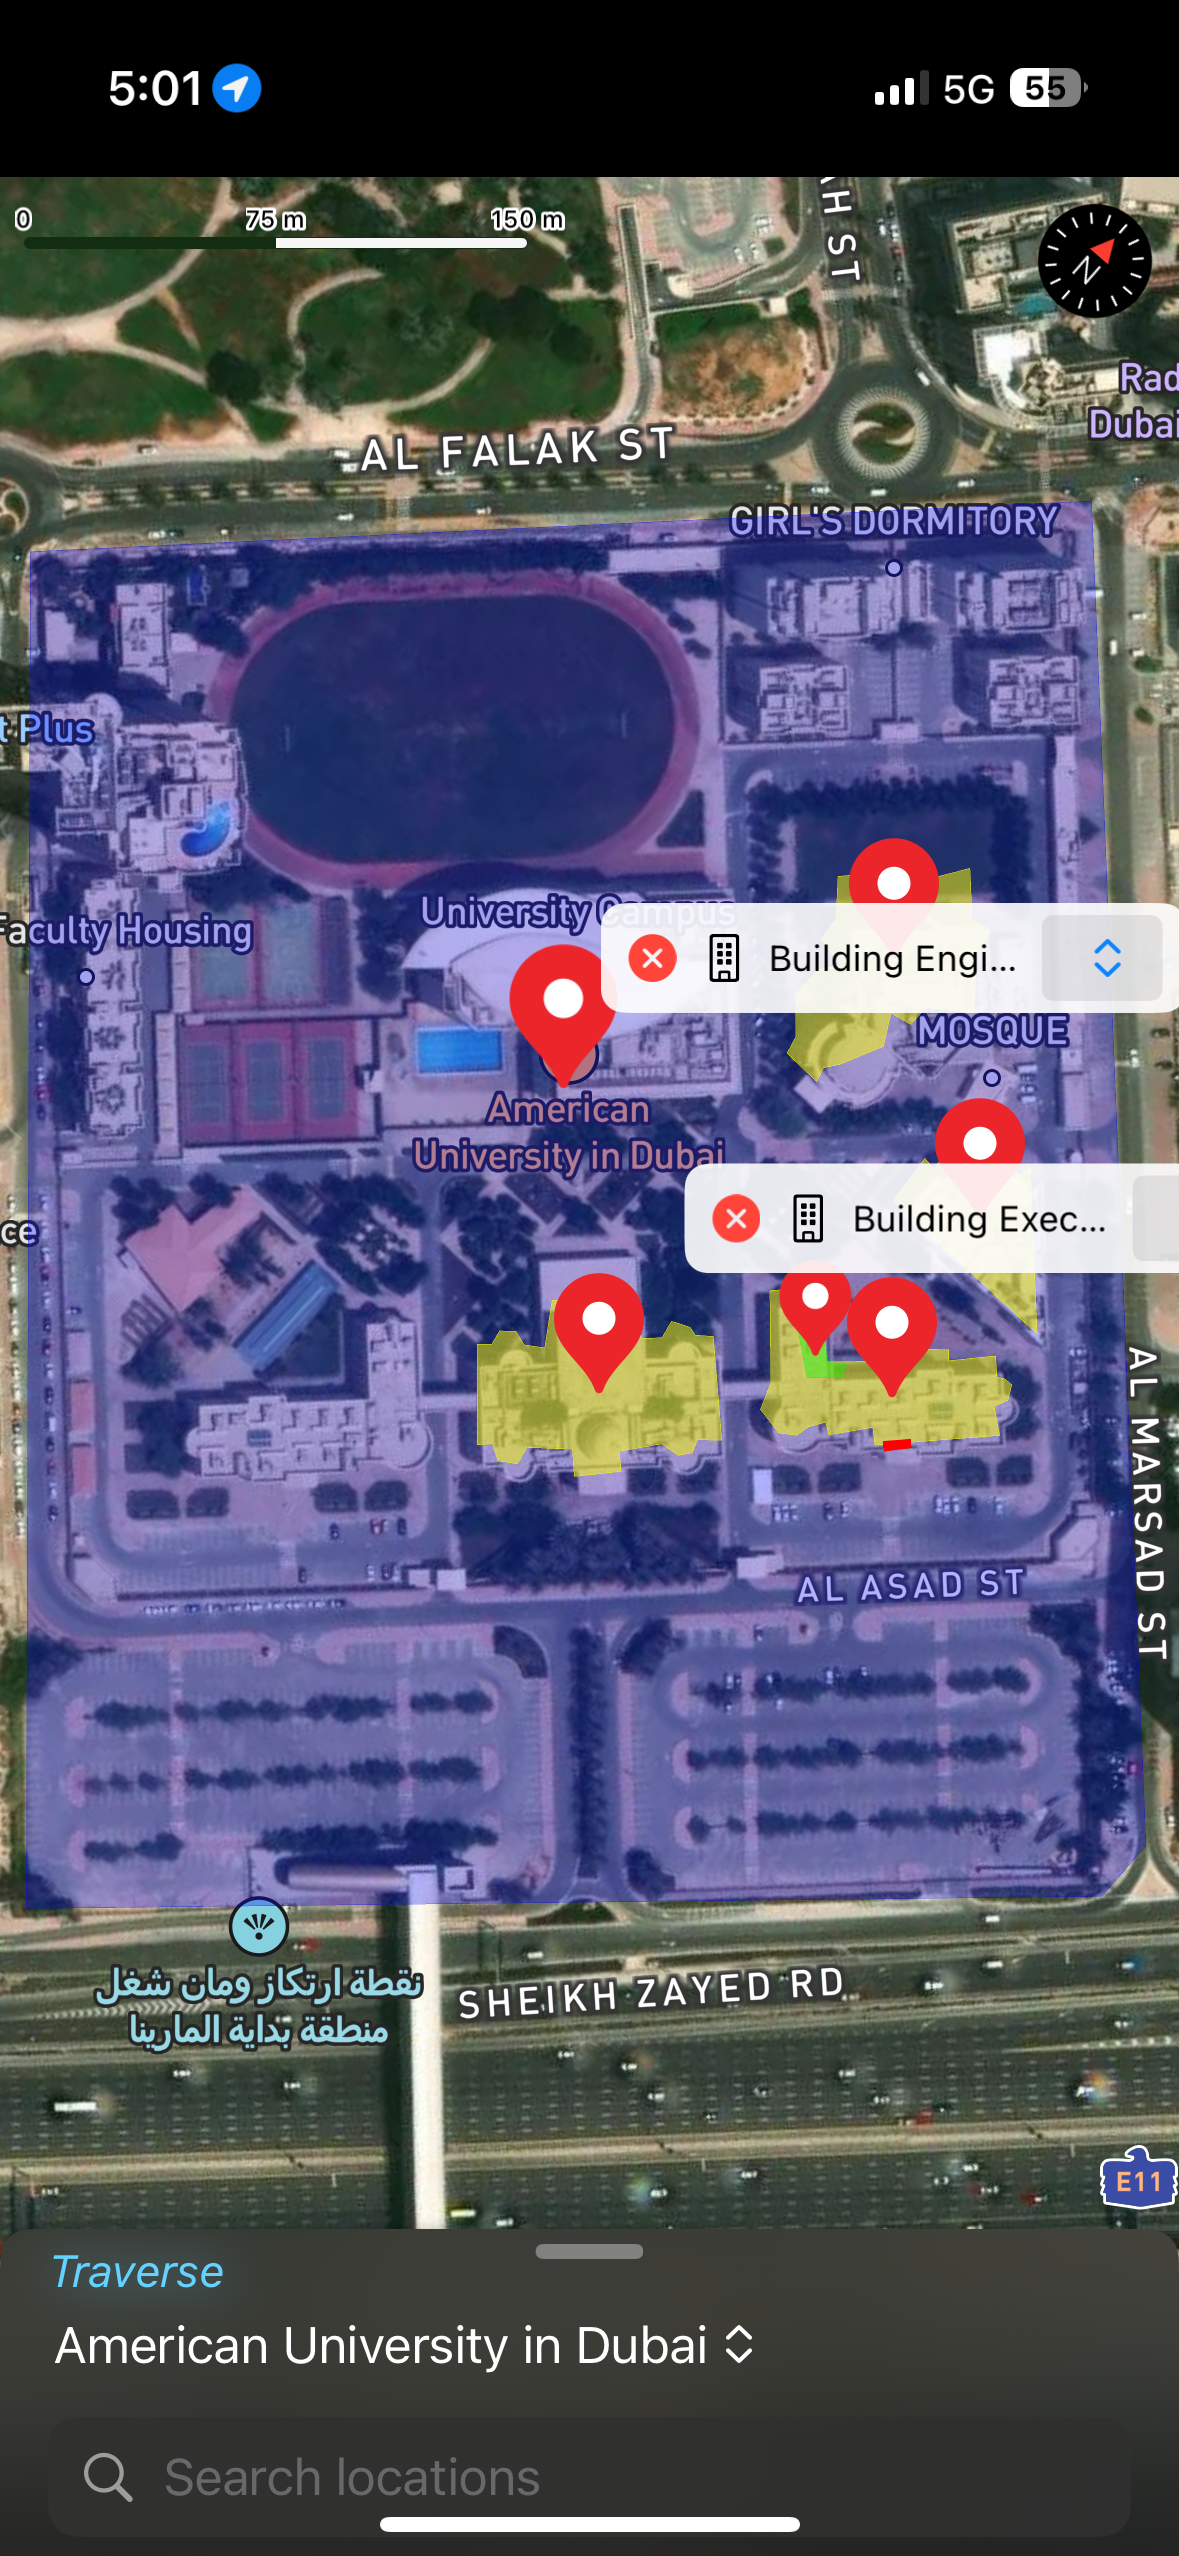
\includegraphics[width=0.8\textwidth]{figures/navigation-route.png}
    \caption{Active navigation showing the shortest path between two locations}
    \label{fig:navigation-route}
\end{figure}

% --- IMDF Data and Implementation ---
\section{IMDF Data Structure}
IMDF (Indoor Mapping Data Format) is Apple's open standard for indoor mapping. For the AUD campus implementation, we utilize the following key components:

\subsection{Core IMDF Components}
\begin{itemize}
    \item \textbf{Venue}: Represents the entire AUD campus as a top-level container
    \item \textbf{Buildings}: Individual structures within the campus
    \item \textbf{Levels}: Floor plans within buildings
    \item \textbf{Units}: Rooms, corridors, and other indoor spaces
    \item \textbf{Amenities}: Points of interest like restrooms, water fountains, etc.
    \item \textbf{Openings}: Doors, stairs, and other transition points
    \item \textbf{Relationships}: Hierarchical connections between different elements
\end{itemize}

\subsection{IMDF File Structure}
Our implementation uses a collection of GeoJSON files:
\begin{verbatim}
data/imdf/AUD.imdf/
    manifest.json      # Dataset metadata
    venue.json        # Campus definition
    building.json     # Building geometries
    level.json       # Floor plans
    unit.json        # Room definitions
    opening.json     # Doors and transitions
    amenity.json     # Points of interest
\end{verbatim}

\subsection{Graph Construction from IMDF}
The navigation graph is constructed by:
\begin{enumerate}
    \item Loading and parsing IMDF files using \texttt{IMDFDecoder}
    \item Creating nodes for each navigable point (unit centers, openings)
    \item Establishing edges between connected spaces
    \item Calculating weights based on real-world distances
    \item Adding accessibility metadata to edges
\end{enumerate}

% --- Internal Architecture ---
\section{Internal Architecture}
\subsection{C++ Graph and Pathfinding}
The core pathfinding logic is implemented in C++ for performance and portability. The `Graph` class represents the campus as a weighted undirected graph, where nodes are locations (e.g., rooms, entrances) and edges represent navigable paths with associated weights (distances or costs). Dijkstra's algorithm is used to compute the shortest path between any two nodes.

\subsection{Swift IMDF Model}
The Swift codebase defines a set of models corresponding to IMDF features (Venue, Building, Level, Unit, etc.). The `IMDFDecoder` loads and parses the IMDF dataset, mapping GeoJSON features to Swift objects. Relationships between features (e.g., which units are on which level) are maintained for efficient querying and navigation.

\subsection{C++/Swift Bridge}
A bridging layer (planned) will expose the C++ pathfinding logic to Swift. This allows the iOS app to request shortest paths by passing node identifiers to the C++ backend and receiving the computed route. This design enables future support for other platforms (e.g., Android) using the same C++ core.

\subsection{SwiftUI Frontend}
The user interface is built with SwiftUI, providing a modern, responsive experience. The main components include:
\begin{itemize}
    \item \textbf{Map View:} Displays the campus map, buildings, and navigation routes.
    \item \textbf{Search Bar:} Allows users to search for locations and amenities.
    \item \textbf{Detail Views:} Show information about selected locations, including accessibility and peak times.
    \item \textbf{Navigation Controls:} Enable users to start navigation and view step-by-step routes.
\end{itemize}

% --- Data Flow and Internal Workings ---
\section{Data Flow and Internal Workings}
\begin{enumerate}
    \item \textbf{IMDF Loading:} On launch, the app loads the IMDF dataset for the selected university. The `IMDFDecoder` parses GeoJSON files into Swift model objects.
    \item \textbf{Graph Construction:} The C++ `Graph` is constructed from the IMDF relationships, with nodes for each navigable location and edges for connections.
    \item \textbf{User Interaction:} Users search for or select a location. The app identifies the corresponding node in the graph.
    \item \textbf{Pathfinding:} When navigation is requested, the app calls the C++ backend (via the bridge) to compute the shortest path between the current location and the destination.
    \item \textbf{Route Visualization:} The computed path is displayed on the map, with step-by-step instructions and accessibility information.
\end{enumerate}

% --- User Manual ---
\section{User Manual}
\subsection{Getting Started}
\begin{enumerate}
    \item Install and launch the Traverse app on your iOS device.
    \item On first launch, select the university campus (currently only AUD is supported).
    \item The main map view will display the campus layout.
\end{enumerate}

\subsection{Searching for Locations}
\begin{enumerate}
    \item Use the search bar at the top to find rooms, amenities, or buildings.
    \item Tap on a search result to view details, including accessibility and peak times.
\end{enumerate}

\subsection{Navigating the Campus}
\begin{enumerate}
    \item Select a location and tap the \textbf{Go} button to start navigation.
    \item The shortest path will be highlighted on the map.
    \item Follow the route to your destination. The app will update your progress in real time.
\end{enumerate}

\subsection{Accessibility Features}
\begin{itemize}
    \item The app displays accessibility information for each location (e.g., wheelchair access, braille signage).
    \item Accessible routes are prioritized in pathfinding where possible.
\end{itemize}

\subsection{Troubleshooting}
\begin{itemize}
    \item If the map does not load, ensure the IMDF data is present in the app bundle.
    \item For navigation issues, verify that your device's location services are enabled.
\end{itemize}

% --- Extensibility ---
\section{Extending Traverse}
\subsection{Adding a New Campus}
\begin{enumerate}
    \item Obtain or generate an IMDF dataset for the new campus.
    \item Add the IMDF files to the app's data directory.
    \item Update the `University` model in Swift to include the new campus.
    \item Rebuild the app; the new campus will be selectable at launch.
\end{enumerate}

\subsection{Adding New Features}
\begin{itemize}
    \item Implement new IMDF feature types by extending the Swift model classes.
    \item Update the UI to display new information or controls as needed.
    \item For new pathfinding logic, extend the C++ `Graph` class and update the bridge.
\end{itemize}

% --- Expanded Code Structure ---
\section{Code Structure}
\begin{itemize}
    \item \texttt{src/Graph.hh, Graph.cc}: C++ graph and pathfinding logic (Dijkstra's algorithm, node/edge management)
    \item \texttt{src/Bridge.hh}: (Planned) C++/Swift bridge interface
    \item \texttt{src/ios/Model/IMDF/}: Swift models for IMDF features (Venue, Building, Level, etc.)
    \item \texttt{src/ios/Model/IMDF/IMDFDecoder.swift}: Loads and parses IMDF data
    \item \texttt{src/ios/View/}: SwiftUI views for the user interface (map, search, detail, navigation)
    \item \texttt{src/ios/ViewModel/}: View models for app state and business logic
    \item \texttt{src/ios/Extension/Geometry.swift}: Geometry helpers for map rendering
\end{itemize}

% --- Code Examples ---
\section{Graph Implementation}

\subsection{C++: Graph Class and Dijkstra's Algorithm}
\begin{lstlisting}[language=cpp]
// src/Graph.hh
#include <vector>
#include <string>
#include <unordered_map>

class Graph {
public:
    Graph();
    ~Graph();
    void addNode(const std::string& node);
    void addEdge(const std::string& from, const std::string& to, double weight);
    std::vector<std::string> shortestPath(const std::string& start, const std::string& end);
private:
    struct Edge {
        std::string to;
        double weight;
    };
    std::unordered_map<std::string, std::vector<Edge>> adjList;
};
\end{lstlisting}

\begin{lstlisting}[language=cpp]
// src/Graph.cc (Dijkstra's algorithm)
std::vector<std::string> Graph::shortestPath(const std::string &start,
                                             const std::string &end) {
    if (adjList.find(start) == adjList.end() ||
        adjList.find(end) == adjList.end()) {
        return {};
    }
    std::unordered_map<std::string, double> distances;
    std::unordered_map<std::string, std::string> previous;
    for (const auto &pair : adjList) {
        distances[pair.first] = std::numeric_limits<double>::infinity();
    }
    distances[start] = 0;
    using P = std::pair<double, std::string>;
    std::priority_queue<P, std::vector<P>, std::greater<P>> pq;
    pq.push({0, start});
    while (!pq.empty()) {
        auto [dist, current] = pq.top();
        pq.pop();
        if (current == end) break;
        if (dist > distances[current]) continue;
        for (const auto &edge : adjList[current]) {
            double newDist = dist + edge.weight;
            if (newDist < distances[edge.to]) {
                distances[edge.to] = newDist;
                previous[edge.to] = current;
                pq.push({newDist, edge.to});
            }
        }
    }
    if (distances[end] == std::numeric_limits<double>::infinity()) return {};
    std::vector<std::string> path;
    std::string current = end;
    while (current != start) {
        path.push_back(current);
        current = previous[current];
    }
    path.push_back(start);
    std::reverse(path.begin(), path.end());
    return path;
}
\end{lstlisting}

\textbf{Explanation:} The C++ code above defines a weighted undirected graph and implements Dijkstra's algorithm to find the shortest path between two nodes. This is the core of the navigation logic.

\subsection{Swift: IMDF Model Parsing and Map Rendering}
\begin{lstlisting}[language=swift]
// src/ios/Model/IMDF/IMDFDecoder.swift
class IMDFDecoder {
    let decoder = JSONDecoder()
    func decode(_ imdfDirectory: URL) throws -> DecodedIMDF {
        let archive = IMDFArchive(directory: imdfDirectory)
        // ...parsing logic for each IMDF feature...
        return DecodedIMDF(
            manifest: manifest,
            venue: venue,
            addresses: addresses,
            levels: levels,
            units: units,
            footprints: footprints,
            relationships: relationships,
            anchors: anchors,
            sections: sections,
            buildings: buildings,
            occupants: occupants,
            amenities: amenities,
            openings: openings
        )
    }
}
\end{lstlisting}

\begin{lstlisting}[language=swift]
// src/ios/View/Component/VenueView.swift
struct VenueView: View {
    @State private var viewModel: VenueViewModel
    @Binding private var viewport: Viewport
    var body: some View {
        Map(viewport: $viewport) {
            ForEvery(viewModel.buildings, id: \.id) { building in
                if let polygon = building.geometry?.asPolygon {
                    PolygonAnnotation(
                        id: building.id.uuidString,
                        polygon: polygon
                    )
                    .fillColor(.yellow)
                    .fillOpacity(0.5)
                }
            }
            // ...other map layers...
        }
        .mapStyle(.standardSatellite(lightPreset: .day))
        .onAppear { viewModel.loadMap() }
    }
}
\end{lstlisting}

\textbf{Explanation:} The Swift code above shows how IMDF data is parsed into model objects and how the map is rendered using SwiftUI. Buildings and other features are displayed as polygons on the map, and the UI updates in response to user interaction.

% --- Future Work and Contributors (unchanged) ---
\section{Future Work}
\begin{itemize}
    \item Complete the C++/Swift bridge for native pathfinding
    \item Add support for more universities and IMDF datasets
    \item Enhance accessibility and real-time data integration
\end{itemize}

\section{Contributors}
\begin{itemize}
    \item Rashid Almheiri
    \item Younis Almazrooqi
\end{itemize}

\end{document}
